\chapter{Bevezetés}
\label{ch:intro}

A szoftverfejlesztés egyik népszerű tautológiája, hogy minőségi, hosszú távon is karbantartható szoftvert fejleszteni rendkívül nehéz. Ennek sok különböző oka, de a probléma központja az, hogy egyszerűen nehéz definiálni, hogy a "jó" és a "minőségi" szavak pontosan mit is jelentenek egy kódbázis esetében. Hiába áll közel a matematika egzakt természetéhez egy kontextus nélkül értelmezett kódsor, minél nagyobb halmazát nézzük távolról egy kódsor halmaznak, annál közelebb kerülünk a filozófiából ismerős minőség erősen homályos koncepciójához.

A tapasztalatra hivatkozhatnánk a minőség egyik prediktoraként, hiszen ha valami bevált korábban több projekten, akkor egy n+1-edik projekten is működni fog. Ez a feltételezés természetesen nem állja meg a helyét. Amellett, hogy a status quo, vagy pontosabban a korábban hozott döntések kritikus vizsgálata előbb fog jó minőségű szoftverhez vezetni, mint annak a vak követése (népszerűbb nevén \textit{cargo cult programozás}), azt is fontos megjegyezni, hogy egy szoftver projekt kontextusának csak egyik vektora a konkrét kód és a mögötte lévő követelmény. A fejlesztő csapat, a csapat és a csapatot alkalmazó cég kultúrája jelentősen torzítják a korábbi tapasztalat alkalmazásának hasznosságát. Melvin Conway programozó 1967-ben tett egy azóta elhíresült kijelentést, amelyre évtizedek óta csak Conway törvényeként\cite{conway} hivatkozunk:
\begin{quotation}
    Any organization that designs a system (defined broadly) will produce a design whose structure is a copy of the organization's communication structure.
\end{quotation}

Conway törvénye azt fogalmazza meg, hogy egy szervezet szoftverei jellemzően tükrözni fogják a szervezet kommunikációs struktúráját. Ez hatással van a korábban említett tapasztalati faktorra: egy szervezetben fejlesztett szoftver és a hozzá tartozó gyakorlatok nem feltétlenül illeszkednek egy másik szervezetben fejlesztett szoftver követelményeire.

Friss vezető fejlesztőként, 2019-ben futottam bele a következő kérdésbe: milyen objektív, empirikus statisztikát alkalmazhatnék egy fejlődő kódbázis elemzésére, ami mentes a saját minőségi kóddal kialakított koncepcióimtól? Ekkor futottam bele az azt megelőző évben megjelent, \textit{Software Design X-Rays}\cite{tornhillXrays} című könyvbe, ami egy számomra új, gyakorlatban hasznosítható megközelítést prezentál a kódbázisokat gyakori problémáinak felismerésére, programozási nyelvtől, paradigmától és platformtól függetlenül.

Az ötlet egyszerű: minden olyan szoftverfejlesztési projekt, ahol a minőség akármilyen szinten releváns, ott a kód verziókezelő rendszerben van tárolva. Ezek a verziókezelő rendszerek nagyon specifikus célokat szolgálnak (erről bővebben az \ref{section:version_control} szekcióban), azonban rengeteg metaadatot tárolnak a kódról projekt, fájl és sor szintjén is.

\citeauthor{tornhillXrays} két statisztikai pontra hivatkozik a könyvében:
\begin{enumerate}
    \item Egy fájl, vagy fájlban lévő sor hányszor került módosításra
    \item Egy fájl, vagy fájlban lévő sor hány különböző szerző által lett módosítva
\end{enumerate}

A feltételezés, hogy a kódbázisok problémás részein kiemelkedően magas lesz a fent említett két szám a kódbázis többi részéhez képest. Továbbá feltehető az is, hogy azok a fájlok, amiken ez megfigyelhető, azok a fejlesztés korai szakaszaitól jelen vannak és a módosítások számának növekedése a projekt életciklusa alatt nagyjából konstans marad.

Jogos kérdés lehet, hogy pontosan miért probléma az, hogy egy fájlt, illetve a benne lévő osztályt gyakran kell módosítani. Ehhez egy pillanatra hátra kell lépnünk és szót kell ejtenünk az úgynevezett code smell-ekről.

\section{Code smell}

A code smell, mint koncepció Martin Fowler \textit{Refactoring}\cite{fowlerRefactoring} című könyvével került be a programozói köztudatba. \textit{Code smell} alatt jellemzően olyan kódot értünk, aminek a működése szigorúan vett értelemben nem helytelen, azonban szoftver dizájn szempontból egészségtelen a kód hosszú távú karbantarthatóságára nézve.

Fowler a könyvében 16 különböző code smell-t definiál, amiből nekünk a következőek relevánsak:
\begin{enumerate}
    \item \textit{Long method}: szükségtelenül hosszú függvény, ami indokolatlanul sok operációt végez, nem fókuszált
    \item \textit{Large class}: indokolatlanul nagy osztály, ami reálisan több különálló osztály logikáját tartalmazza. Gyakorlatban \textit{God Class} vagy \textit{God Object} néven hivatkozunk erre a code smell-re
    \item \textit{Divergent change}: egy változtatás végrehajtásához sok, egymástól független függvény megváltoztatása szükséges
    \item \textit{Shotgun surgery}: egy kis változtatás sikeres végrehajtása csak sok osztály megváltoztatásával lehetséges
\end{enumerate}

Fontos megjegyezni, hogy a code smell, mint olyan, pusztán egy felületi heurisztika: egy kódrészlet, amire egy, vagy akár több code smell is illeszkedik, az a saját kontextusában lehet dizájn szempontból is helyes, hiszen minden szoftver projekt más. Az code smell-ek értéke abban rejlik, hogy a segítségükkel gyorsan fel tudunk ismerni gyakran előforduló, problémás mintákat, majd egyéni mérlegelés után dönthetünk arról, hogy szükséges-e változtatást eszközölni a gyanús kódon.

\section{Verziókezelő}
\label{section:version_control}

A verziókezelő szerves részeit képzik a modern szoftverfejlesztésnek. A fejlesztői körökben híres \textit{Joel Test}\footnote{\url{https://www.joelonsoftware.com/2000/08/09/the-joel-test-12-steps-to-better-code/}} legelső lakmusz-tesztje, hogy egy projekt minden forráskódjának valamilyen formában verziókezelőben kell lennie, máskülönben (Spolsky véleménye szerint) a fejlesztők csak a saját és a klienseik életét nehezítik meg.

De mi is pontosan egy verziókezelő? Egy verziókezelő szoftver célja, hogy a forráskódon történő változtatások mindig világosan visszakövethetőek legyenek, egyértelműen látszódjon a változtatás előtti és utáni állapot és a forráskód akármelyik állapota akármikor elérhető és visszaállítható legyen. Fontos továbbá az is, hogy a verziókezelő rendszerek úgynevezett branch-ek használatával elősegítik, hogy egy fejlesztő csapat minden tagja képes legyen ugyanazokon a fájlokon más-más változtatásokat végrehajtani úgy, hogy a potenciálisan létrejött konfliktusokat csak egyszer kell feloldani.

Koncepcionálisan a verziókezelőket, illetve az azokban tárolt forráskódot nagyon komplex gráfként érdemes elképzelni, amelynek minden csúcsa a forráskód egy bizonyos állapota.

A legismertebb verziókezelők:
\begin{itemize}
    \item \textit{SVN}: a 2000-es évek elejének legnépszerűbb, centralizált verziókezelő rendszere.
    \item \textit{Perforce}: centralizált verziókezelő, ami koncepcionálisan az SVN-hez közelít, azonban nem nyílt forráskódú. Nagy céges környezetben a mai napig viszonylag népszerű, köszönhetően főleg annak, hogy kiválóan képes kezelni a bináris fájlokat.
    \item \textit{git}: messze a legnépszerűbb modern, decentralizált verziókezelő rendszer. Bővebben részletezve a következő szekcióban.
\end{itemize}

Terminológia szempontjából a következők lesznek fontosak:
\begin{itemize}
    \item \textit{Repository}: egy megosztott adatbázis, ami tartalmazza a verziókezelt forráskód összes különböző verziójának állapotát
    \item \textit{Commit}: változtatások egy halmaza, ami a forráskód egy korábbi változatát egy új verzióra képezi le
    \item \textit{Branch}: a forráskód egy bizonyos commit-járól való leágazás, ami egy, a szülő branch-től független commit történettel fog rendelkezni a vágási ponttól
    \item \textit{Author}: egy commit változtatásaihoz rendelt szerző
\end{itemize}

\subsection{A legnépszerűbb verziókezelő - git}\label{section:git}

A git fejlesztése 2005-ben indult Linus Torvalds vezetésével, miután a Linux kernel által használt zárt forráskódú BitKeeper verziókezelő rendszer fizetőssé vált. Ebben az érában a verziókezelő rendszerek a zárt forráskód-kiforrott funkcionalitás, nyílt forráskód-kiforratlan funkcionalitás párosok által képzett két halmazba tartoztak.

A git dizájnját a BitKeeper pozitívumai vezérlték: a merge és fork operációk legyenek egyszerűen végrehajtható műveletek, ellentétben a fő versenytársakkal, mint a CVS és az SVN, ahol többek között a materializált branch-ek nehezítették ezeket a műveleteket.

Az igazi áttörést a git-nek a 2008-ban alapított GitHub hozta meg: a 2008-as és 2014-es évek között a GitHub-on tárolt repository-k száma exponenciálisan növekedett évről évre. 2014-re a git beérte az SVN-t, 2020-ra pedig már közel háromszor annyi git-en tárolt repository-t tartott számon a nyílt forráskódú közösség, mint SVN-en.

\begin{figure}[H]
    \centering
    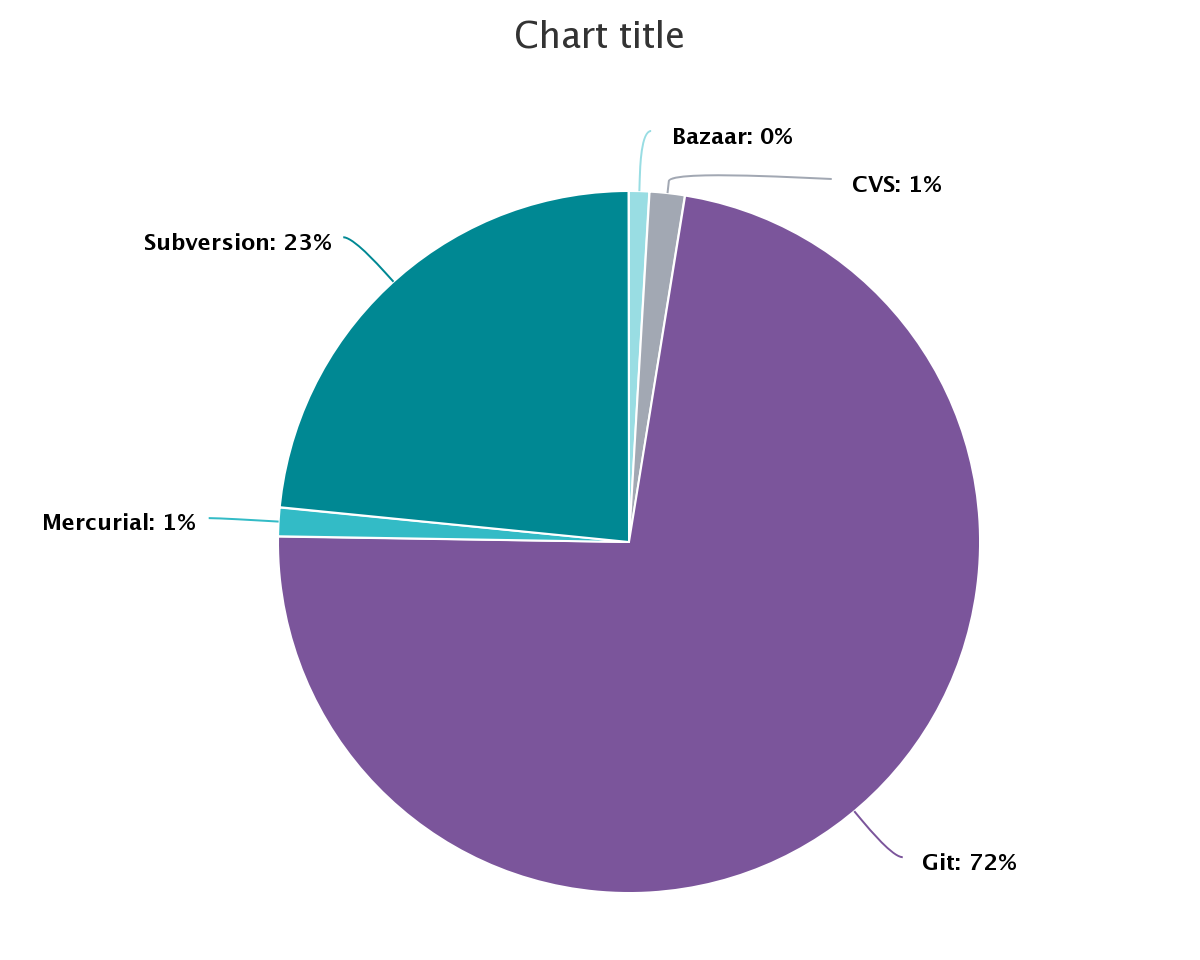
\includegraphics[width=0.8\textwidth]{images/gitMarketShare.png}
    \caption{Verziókezelők relatív népszerűsége 2020-ban}
    \label{fig:version-controls}
\end{figure}

\begin{figure}[H]
    \centering
    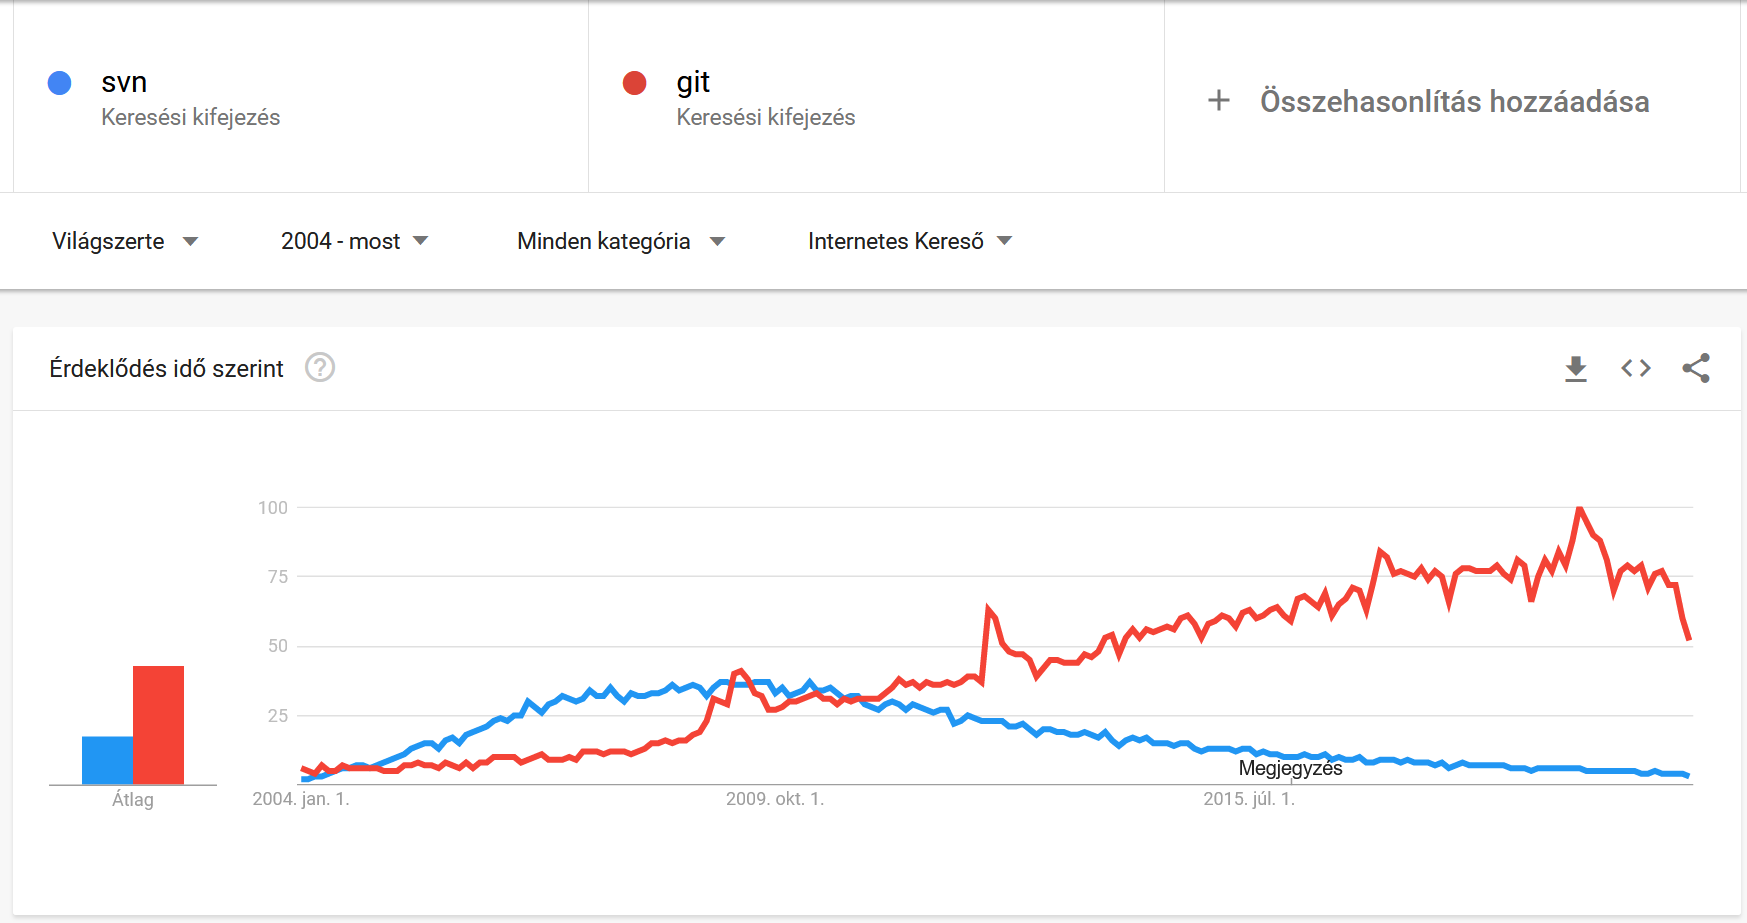
\includegraphics[width=0.8\textwidth]{images/gitsvn.png}
    \caption{A git és SVN népszerűségének változása Google Trends szerint 2004 és 2020 között}
    \label{fig:git-svn-trends}
\end{figure}


Manapság a git a de facto verziókezelő rendszer mind ipari, mind nyílt forráskódú környezetekben, amitől csak nagyon specializált esetekben szokás eltérni -- ilyenek például az egyes tech óriások monorepository-jai, amik a cég teljes forráskódját hivatottak tárolni (ezek a cégek általában saját fejlesztésű verziókezelőt használnak), vagy az olyan projektek, ahol binárisok is verziókezelve vannak (a git teljesítményét már viszonylag kis mennyiségű követett bináris is nagyon érzékenyen érinti).

Korábban már tisztáztunk pár alapvető koncepciót a verziókezelőkkel kapcsolatban, azonban a git megértéséhez pár másikról is szót kell ejteni.

\begin{itemize}
    \item \textit{Decentralized Version Control}: decentralizált verziókezelő alatt azt kell érteni, hogy minden fejlesztő gépén egy teljes értékű repository található, ami képes teljesen önálló működésre központi szerver nélkül. Ez szöges ellentéte például a Perforce-nak, ahol a depo és a fejlesztő gépén lévő repository között gyakorlatilag folyamatos interakcióra van szükség
    \item \textit{Working copy}: egy git repository másolata
    \item \textit{Staging area}: a working copy-n végrehajtott változtatásokat a staging area-ba kell mozgatni, mielőtt azok egy commit-ba kerülhetnek, tehát egy
    \item \textit{Remote}: egy, a lokálistól különböző git repository, aminek a branch-eivel a push és pull műveletekkel tudunk interakcióba lépni. Fontos, hogy egy remote koncepcionálisan nem egy központi repository-t jelent, még akkor sem, ha gyakorlatban az szokott lenni -- egy remote lehet akár csak egy lokálisan tárolt másik másolata a repository-nak, a lényeg, hogy git repository legyen
    \item \textit{Push}: "toljuk fel" a lokális history-t a push-nak megadott távoli branch felé
    \item \textit{Pull}: a push-al ellentétes művelet. Húzzuk le a remote egy adott branch-éről az ott lévő history-t a working copy-ba.
\end{itemize}

\subsection{Code smell-ek nyomai a verziókezelőkben}

Itt az ideje részleteiben kitérni a \textit{Software Design X-Rays}\cite{tornhillXrays} kapcsán már említett git statisztikákra. Ugyan korábban és a későbbiekben is git statisztikaként hivatkozom az itt prezentált statisztikákra, azt fontos itt megjegyezni, hogy ezek tökéletesen alkalmazhatóak akármelyik másik verziókezelő szoftverre is, ami érti valamilyen formában a commit, history és author koncepciókat. A git azonban, ahogy a \ref{section:version_control} fejezet taglalta, messze a legnépszerűbb veriókezelő rendszer 2020-ban, ezért már csak statisztikai alapon is erre esik a választás.

\textit{Khohm et al.}\cite{khomh} kutatása négy ipari projekt vizsgálatán keresztül demonstrálta, hogy az olyan osztályok, amik code smell-eket mutatnak, azok az életciklusuk során lényegesen több változtatást vonzanak magukhoz, mint a nem-problémás fájlok.

Továbbá \textit{M. Tufano et al.} "When and Why Your Code Starts to Smell Bad"\cite{codeSmells} című kutatása azt vizsgálta, hogy a code smell-ek mikor és hogyan kerülnek be egy kódbázisba. A konklúzió a következő lett:
\begin{enumerate}
    \item Az esetek jelentős többségében a code smell-ek az osztályok születésétől jelen vannak, ellentétebn a közhiedelemmel, miszerint a kód evolúciójának a következményei
    \item A code smell-től szenvedő osztályok és fájlok más fejlődési trendeket mutatnak, mint a "tiszta" társaik
    \item A code smell-ek jellemzően új feature-ök fejlesztése közben kerülnek be a kódbázisba, azonban a mintában nem inszignifikáns mennyiségű code smell került be refactor-t tartalmazó commit-okban
    \item A code smell-ek bevezetése általában olyan fejlesztőkhöz köthetőek, akik magas terhelés alatt vannak
\end{enumerate}

Ezekből a tanulságokból kifejezetten a 2-es pontot fogjuk megvizsgálni a \ref{ch:results} fejezetben.

\section{Tesztelés}

A szoftverfejlesztés egyik nagy előrelépése az volt, hogy sikerült már az átlag fejlesztő fejébe is beültetni azt az egyszerű gondolatot, hogy az automatizált tesztelés minden projekten kritikus. Továbbá azt is egyre többen kezdik megérteni, hogy a teszt kód ugyanannyira fontos, mint az éles kód: a tesztek egyfajta kettős könyvelésként működnek a szoftverfejlesztés világában.

\begin{figure}[H]
    \centering
    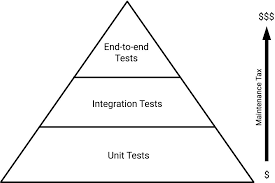
\includegraphics[width=0.8\textwidth]{images/piramis.png}
    \caption{Tesztelési piramis}
    \label{fig:testing-pyramid}
\end{figure}

Az automatizált tesztelésnek több különböző szintje van, amit a \ref{fig:testing-pyramid} ábrán látható tesztelési piramis is mutat. Röviden ezekről a tesztelési szintekről lesz most szó.

\subsection{Magasabb szintű tesztek}

A tesztelési piramis legfelsőbb szintjén találjuk az E2E, azaz end-to-end teszteket. E2E teszt alatt, ahogy a neve is mutatja egy olyan tesztet értünk, ami a teljes szoftvert teszteli, jellemzően vagy egy UI-ról vagy egy REST endpoint-ról elindulva. Az automatizált UI tesztek egy specializált, nagyon gyakran alkalmazott variánsát képezik az E2E teszteknek -- ezekkel azt lehet elérni, hogy a szoftver belső működésének ismerete nélkül teszteljük úgy a teljes szoftvert, mintha a felhasználók kezében lenne.
A webes világban például a Selenium, WebDriver és Cypress segítségével leírhatjuk, hogy a tesztek milyen elemeket keressenek egy weboldalon, milyen interakciókat végezzenek ezeken az elemeken, illetve minek kell történnie az interakciók hatására.

Közvetlenül az E2E tesztek alatt helyezkednek el az integrációs tesztek. Az integrációs tesztek abból a szempontból hasonlítanak az E2E tesztekre, hogy a céljuk valamilyen szinten éles körülmények között tesztelni a kódbázis több rétegét. Az éles körülmények alatt jellemzően azt kell érteni, hogy a kód és egy külső erőforrás integrációját tesztelik.
Például képzeljük el azt, hogy szeretnénk ellenőrizni, hogy a web service-ünk a megfelelő sorokat szúrja be a vele kapcsolatban álló adatbázissal. Ezt egy unit tesztben úgy ellenőriznénk, hogy az adatbázis absztrakció megfelelő függvényét ellenőriznénk, hogy meg lett-e hívva. Egy integrációs teszt esetében ugyanezt úgy ellenőrizzük, hogy magán az adatbázison nézzük meg, hogy az adott sor bekerült-e.

\begin{figure}[H]
    \centering
    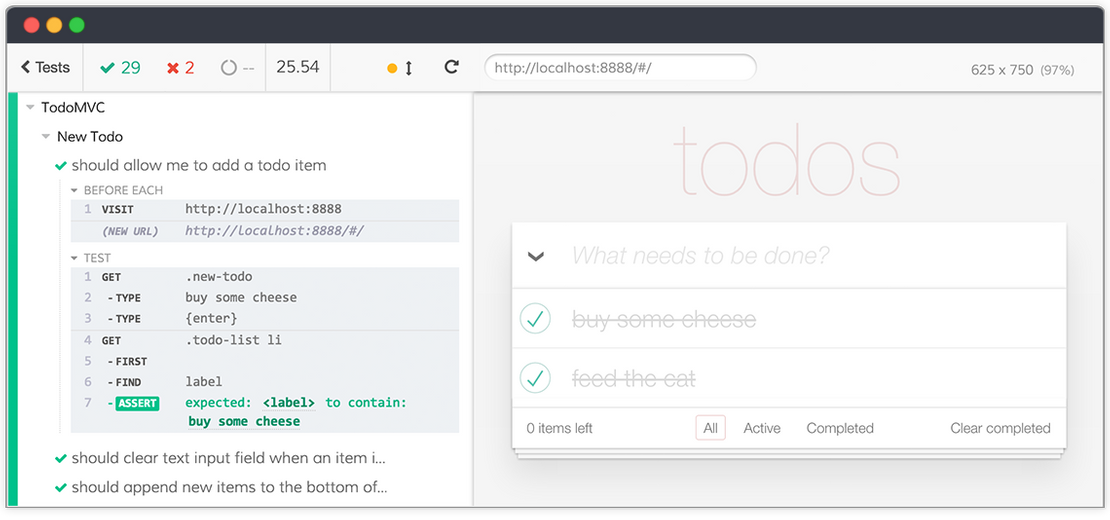
\includegraphics[width=1\textwidth]{images/cypress.png}
    \caption{Egy Cypress-ben futtatott E2E teszt}
    \label{fig:cypress-example}
\end{figure}

\subsection{Unit tesztelés}

A tesztelési piramis legalsó szintjén található a unit tesztelés. \textit{Unit teszt} alatt egy olyan tesztet értünk, ami izolációban teszteli egy nagyon specifikus részét a kódnak. Izoláció alatt itt azt értjük, hogy a tesztelt egység függőségei mock-olva vannak, azaz teszt objektumokra vannak cserélve.

A pontos definíció ebben az esetben kissé vitatott, mert gyakorlatban a unit tesztelésnek több különböző stílusa létezik. Jellemzően ezek a stílusok eltérnek az izoláció mértékében, a tesztelt kód specificitásában és az ellenőrzések formájában is. Sok projekt továbbá kombinálja ezeket a különböző stílusokat az alkalmazás különböző rétegeiben.

Definíciótól függetlenül azonban a unit tesztek célja világos: bizonyítsuk, hogy a kód, amit írtunk tényleg úgy viselkedik, ahogy szeretnénk és ez a verifikáció legyen könnyen és gyorsan megismételhető.

Ellentétben a korábban már említett E2E tesztekkel, a unit tesztek fehér doboz tesztek, ami azt jelenti, hogy a teszt maga részleteiben ismeri a tesztelt kódot, hiszen direkt interakcióban van vele.

\begin{figure}[H]
    \centering
    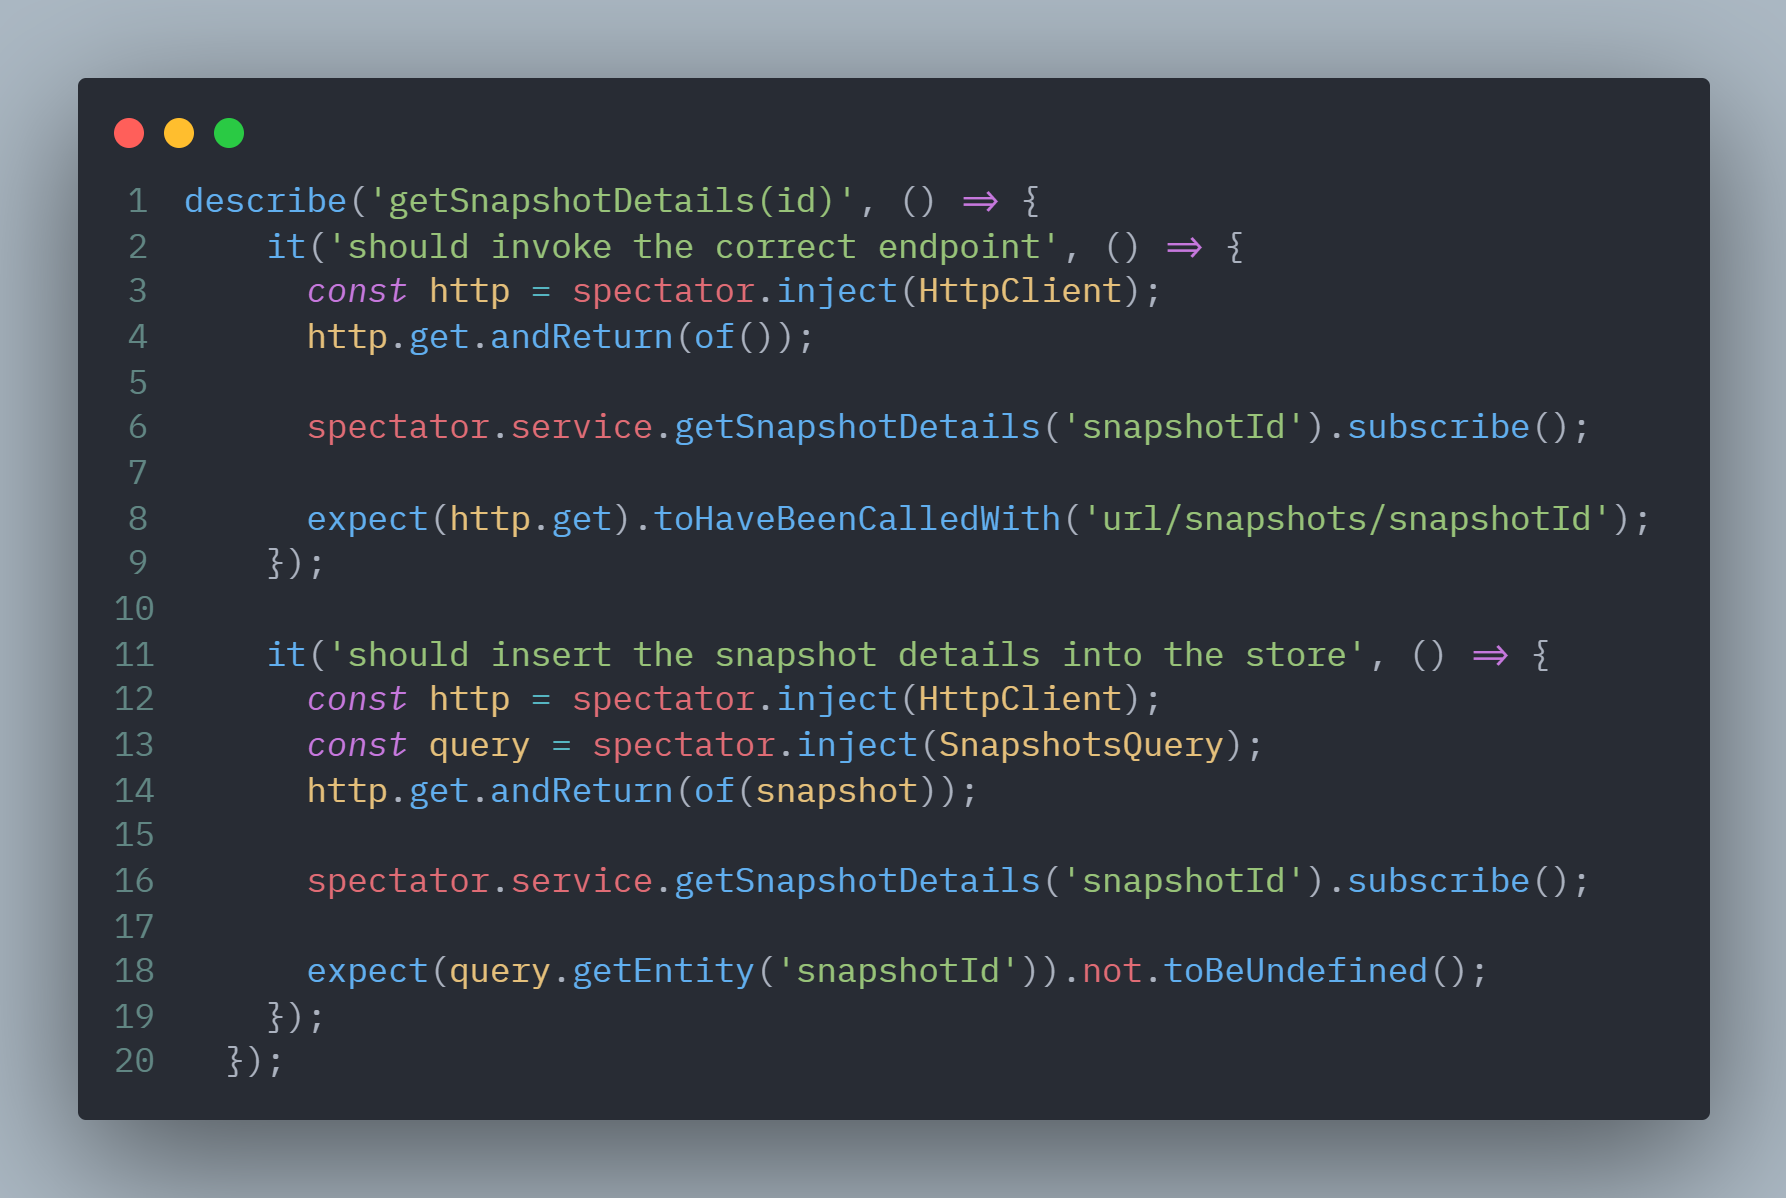
\includegraphics[width=0.8\textwidth]{images/unit-test.png}
    \caption{Unit teszt a Hestia UI projektből}
    \label{fig:unit-test-example}
\end{figure}

\begin{figure}[H]
    \centering
    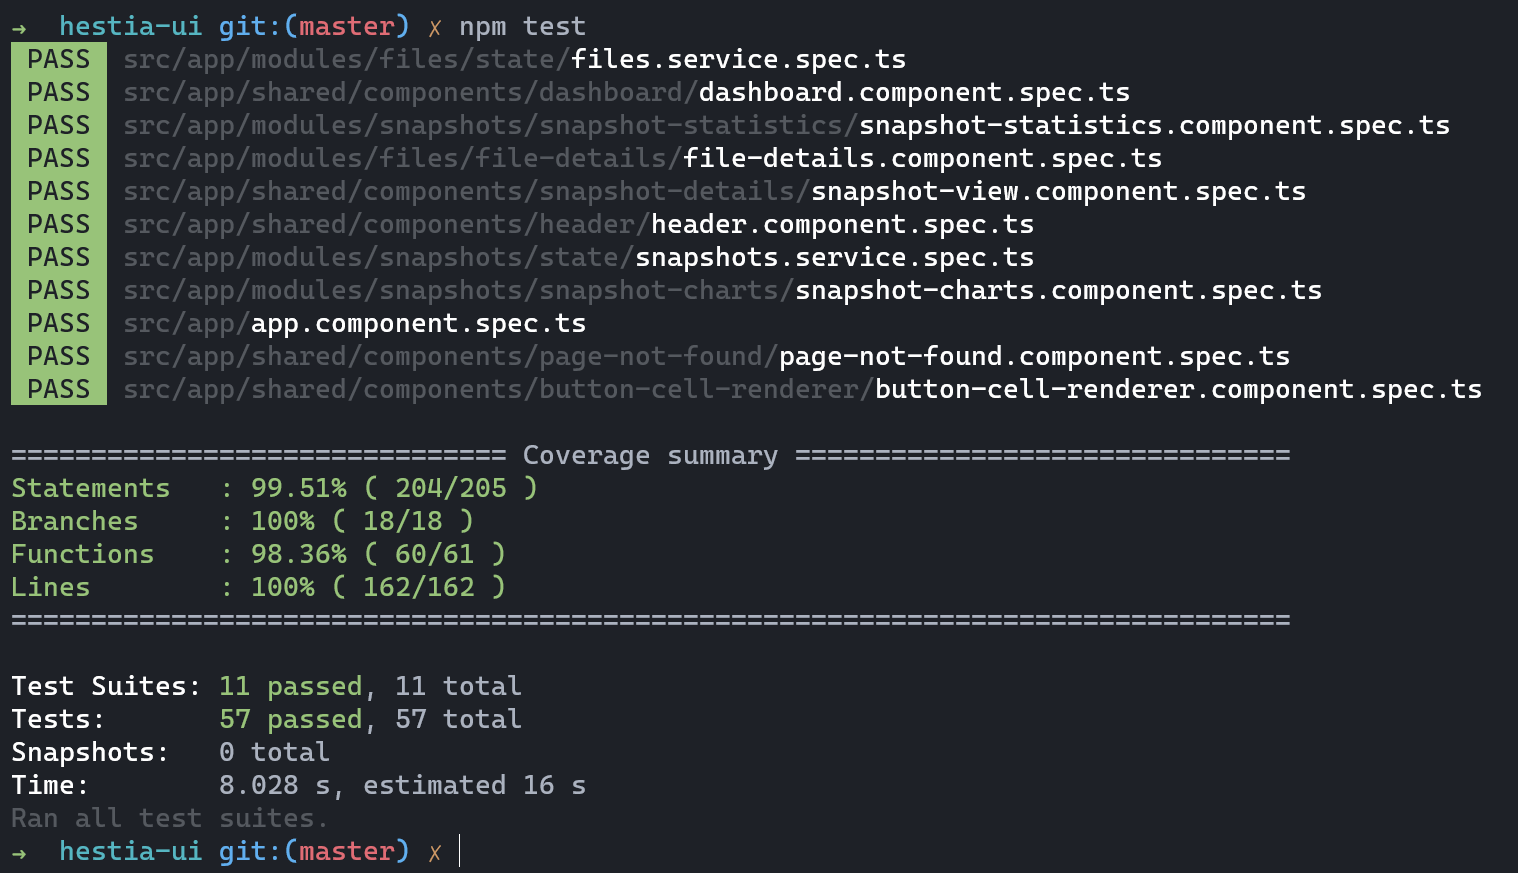
\includegraphics[width=0.8\textwidth]{images/testRun.png}
    \caption{Unit tesztek futtatása}
    \label{fig:unit-test-run-example}
\end{figure}

\section{Teszt coverage}

Tisztáztuk a korábbiakban a tesztelés alapvető célját és a különböző szintjeit, azonban arról még nem esett szó, hogy milyen metrikákat tudunk kinyerni egy kódbázis tesztjeiből. Itt jön képbe a teszt coverage, ami azt mutatja, hogy a futattott tesztek milyen arányban hajtják meg az éles kódot, bizonyos szempontok szerint. Jellemzően a következő különböző szinten értelmezzük a coverage-et:
\begin{itemize}
    \item \textit{Statement coverage}: a kódbázis kifejezéseinek coverage értéke
    \item \textit{Line coverage}: a kódbázis konkrét, tényleges kódot tartalmazó sorainak coverage értéke
    \item \textit{Function coverage}: a kódbázisban függvényeinek coverage értéke
    \item \textit{Branch coverage}: vezérlési struktúrák ágainak coverage értéke
    \item \textit{Condition coverage}: a kódbázisban talált boolean vezérlési struktúrák feltételeinek coverage értéke
\end{itemize}

\begin{figure}[H]
    \centering
    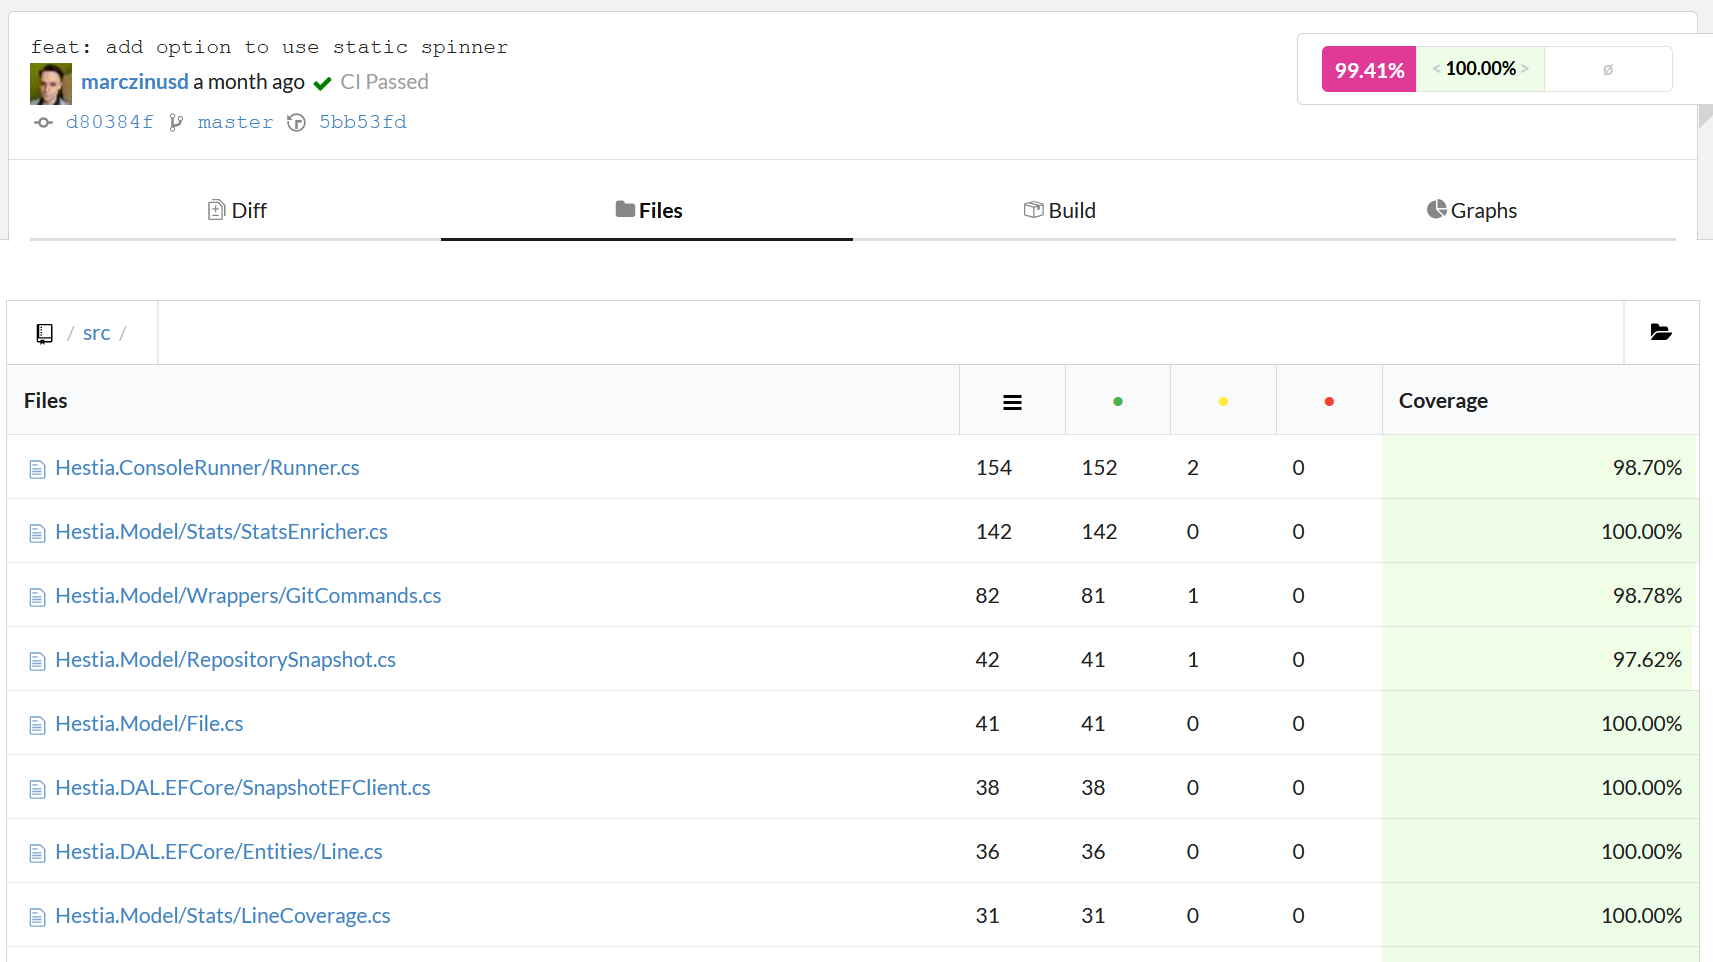
\includegraphics[width=1\textwidth]{images/codecov-report.png}
    \caption{Egy coverage report a codecov.io oldalról}
    \label{fig:codecov-example}
\end{figure}

Technikailag a tesztelési piramis minden szintjéből generálható coverage report, de ahogy haladunk felfelé a hierarchiában, ez egyre nehezebb és kevésbé releváns lesz.

\subsection{Kódminőség és a teszt coverage}

A coverage gyakran kerül említésre, mint egy mérce, ami valamilyen mértékben reprezentálja a kódminőséget. Felmerülhet azonban a kérdés, hogy a code coverage valóban mércéje-e a kódminőségnek. Több kutatás \cite{onRelation}\cite{singhkochhar:hal-01653728} vizsgálta azt, hogy milyen kapcsolatban áll a code coverage és a kódminőség, ahol a kódminőség alatt ebben az esetben a szoftverhibák alacsony számát értjük. Ezek a kutatások azt mutatják, hogy a korreláció a coverage és a minőség között alacsony. A "Mythical Unit Test Coverage"\cite{mythical} továbbviszi ezt az ötletet és a code coverage-et a változtatások komplexitásával párosítja, hasonló eredménnyel, mint a korábbi kutatások: a code coverage önmagában nem elégséges metrika a kódminőség meghatározására.

Az előbbiekből könnyen levonhatnánk konklúzióként, hogy a coverage kódminőségi metrikaként való használata legjobb esetben is spekulatív, hiszen több kutatás mutat abba az irányba, hogy a korreláció a kódminőség és a coverage között valahol a nem létező korreláció és a gyenge korreláció között van, amennyiben a kódminőséget abban mérjük, hogy mennyi hiba képes bekerülni egy éles szoftverbe.

Reálisan nézve viszont sem a kódminőség, sem maga a szoftverfejlesztés nem ennyire egzakt. Akárki, aki dolgozott legacy projekten tisztában van azzal, hogy mekkora a különbség egy olyan kódbázis között, ahol a legkisebb refactor-t is lehetetlen automatizáltan tesztelni és egy olyan között, ahol minden osztályt fed legalább egy pár viszonylag triviális teszt. Nyilvánvaló, hogy a code coverage önmagában egy gyenge metrika, azonban egyéni, fejlesztői szempontból a különbség egy 50\%-os és egy 98\%-os code coverage-el rendelkező projekt között távolról sem marginális.

A unit tesztelés és így a coverage hatása a sokkal kevésbé mérhető fejlesztői kultúrában manifesztálódik és csatlakozik ebben az aspektusában a statikus kódelemző eszközökhöz, mint a SonarQube\footnote{\url{https://www.sonarqube.org/}}, vagy a webes világból ismert linter-ek\footnote{\url{https://eslint.org/}}. Mind a unit tesztelésnek, mind a statikus kódelemzésnek a gyakorlati hatása sokkal könnyebben észrevehető, ha egy projekt karbantarhatóságát nézzük. A teszteknek a hiánya nagyon könnyen képes olyan fejlesztői környezethez vezetni, ahol az emberek félnek változtatni olyan kódon, amikre egyrészt nincs teszt, másrészt a kód mögötti pontos követelmény már nem világos. Ezzel szemben egy jól tesztelt kódbázis egy bizonyos szinten dokumentálja saját magát. Az E2E tesztek a felhasználók elvárásait, az integrációs tesztek a szoftver éles körülményeit, a unit tesztek pedig a fejlesztők mikrodöntéseit kommunikálják.

Érdemes tehát a code coverage-re a karbantarhatóság \textbf{egyik} metrikájaként gondolni.

\section{A teszt coverage és git statisztikák közös vizsgálata}

Most, hogy körbejártuk mind a git statisztikákat, mind a tesztelési kérdéseket és metrikákat, itt az ideje arról is szót ejteni, hogy pontosan mit fog ez a diplomamunka vizsgálni és mi a feltételezés.

Azt könnyű belátni, hogy mind a git statisztikák, mind a code coverage hasonló koncepciókkal dolgoznak (fájl- és sorszintű, könnyen mérhető és szemrevételezhető heurisztikák), így kézenfekvő ötletnek tűnik a kettő együttes vizsgálata. A vizsgálat célja, hogy egyrészt maguknak a git statisztikáknak az evolúcióját próbáljuk értelmezni a kódbázisok élettartama alatt és ebből vonjunk le következtetéseket. A másodlagos cél az az, hogy nézzük meg milyen kapcsolatban áll a git statisztikák alakulása a teszt coverage-el. Van-e moderáló hatása a teszt coverage-nek a gyakran változtatott fájlokon? Hogy alakul a coverage ezeken a fájlokon -- konstans marad, romlik, vagy esetleg nő?

Mielőtt ezeket a kérdéseket megvizsgálnánk, először nézzük meg a probléma vizsgálatára írt programokat.